\documentclass[a4paper]{article}
\usepackage{amsmath}
\usepackage{amssymb}
\usepackage{geometry}
\usepackage{natbib}
\usepackage{float}%稳定图片位置
\usepackage{graphicx,subfig}%画图
\usepackage{caption}
\usepackage[english]{babel}
\usepackage{indentfirst}%缩进
\usepackage{enumerate}%加序号
\usepackage{multirow}%合并行
\usepackage{hyperref}
\usepackage{verbatim}
\title{\Large \textbf{SI649 Lab2}\\
\author{\textbf{Chongdan Pan}\\
uniqname: pandapcd
}
}
\begin{document}
\maketitle
\section{Good Vis}
\begin{figure}[H]
    \centering
    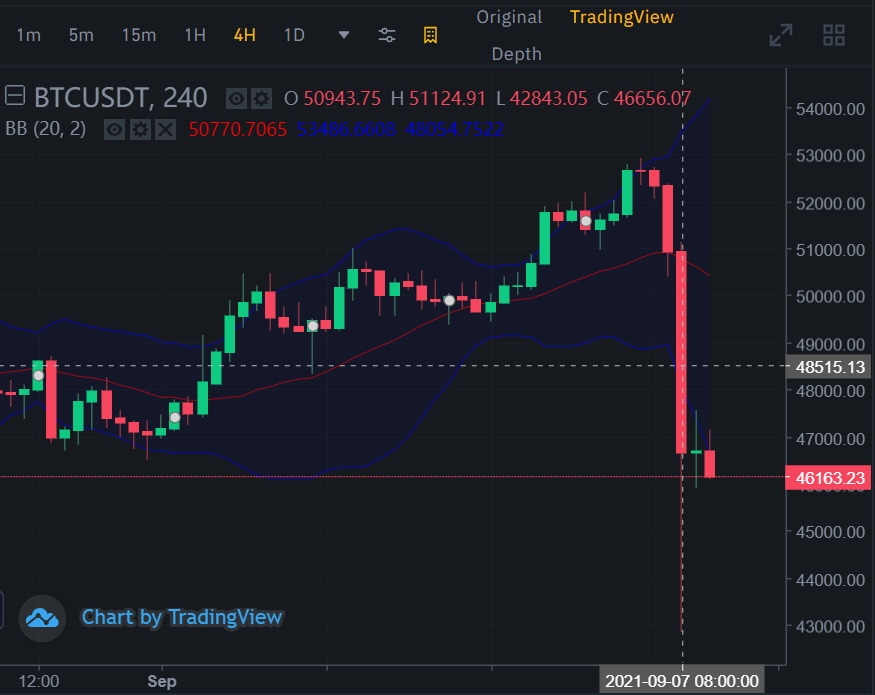
\includegraphics[scale=0.4]{BTCUSDT.png}
    \caption{BTCUSDT trading view from Binance}
\end{figure}
I think the trading view of BTC/USDT from Binance is a good and excellent visualization. It uses a candlestick chart to show the price of BTC/USDT in past. Each candlestick shows the price movement in certain time interval with equal length in the past, where its color shows whether the price goes up or goes down, and its shadow shows the highest and lowest price in this interval. This is a good visualization because compared to a line, the candlestick negelects unnecessary details like subtle fluctuation and keeps most important information in past, so that we can view the price in a longer time range. 
\par The candlestick itself is only for qualitative analysis, so well labeled axis is also included in the chart. The right and bottom axis shows the price and timestamp of specific candlestick, and the top label shows its open, close, high, low price. These labels give us a more specific data and quantative information.
\par In addition, the chart also adds bollinger bands to the candlestick chart. The bollinger shows the move average and track calculated by average and standard deviation. Thanks to different reperesentation of candlestick and bollingband, the viewer can tell the difference between them and find out the outliers directly.
\section{Bad Vis}
\begin{figure}[H]
    \centering
    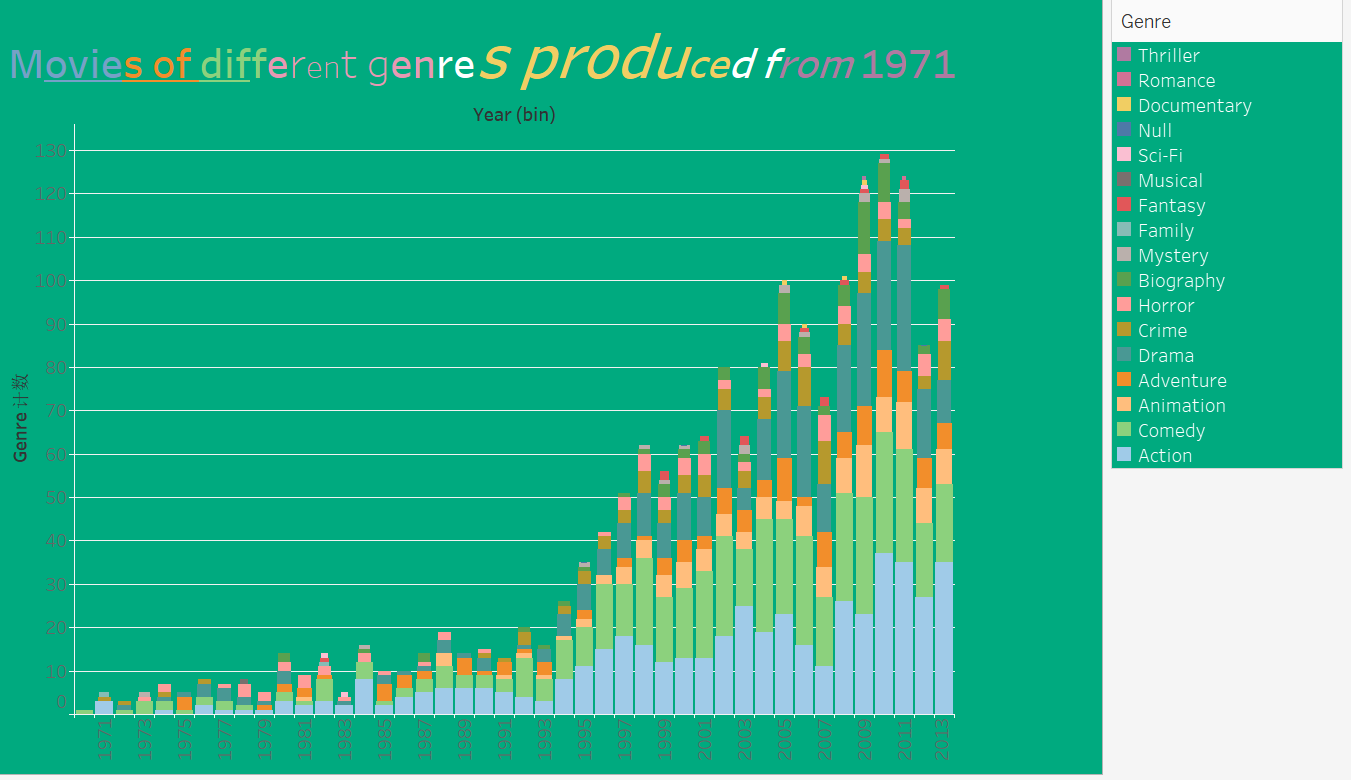
\includegraphics[scale=0.4]{UglyVis.png}
    \caption{UglyVis of data about movies}
\end{figure}
I create the ugly visualization chart from data of lab 2.This chart shows the number of movies of different genres from 1971 to 2013. This chart still has usage because it does show the information that I want to express. However, it's extremely ugly for me, and there are many reasons for it.
\par Firstly, there are too much bars so that it's hard for the user to find data in the year that we want, and the bars are too narrow. Secondly, there are also too much color and the colors are quite inharmonious. The background color is similiar to that used in bars. Thirdly, the title is also very ugly, because if composed words of different color, different size and different style. Forthly, the different part of each bar has different width, it's also very ugly.

\end{document}